\newpage
\graphicspath{{../suyluancungbi/sudoku1/}}
\begingroup
\AddToShipoutPicture*{\put(62,600){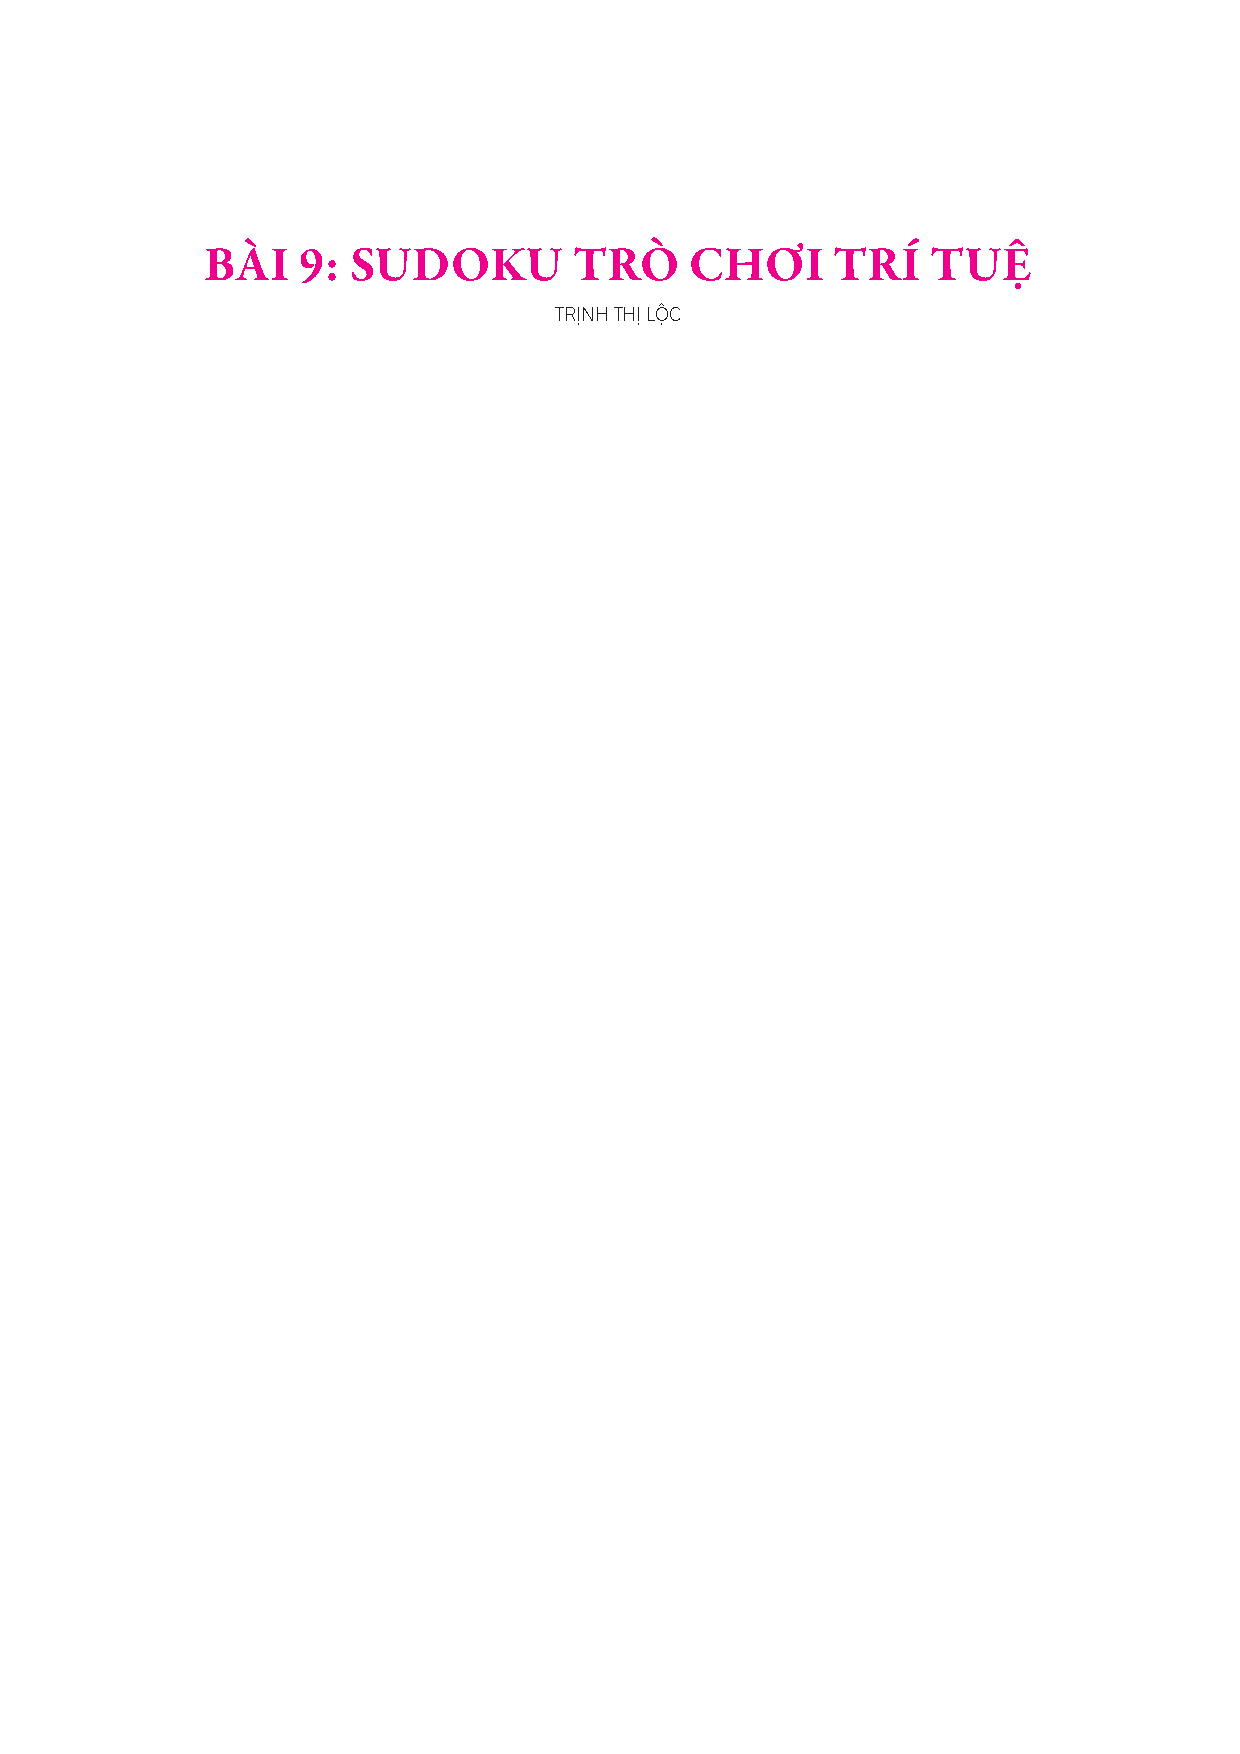
\includegraphics[scale=1]{../sudoku1/sudokutieude1.pdf}}} % %Image background
\centering
\endgroup
\vspace*{20pt}

	\begin{multicols}{2}
		\textbf{Sudoku}, ban đầu có tên gọi là \textbf{Number Place}, là một trò chơi với câu đố điền các số vào các ô trống của một bảng ô vuông có $9$ hàng và $9$ cột (gọi vắn tắt là bảng $9\times 9$), sao cho trong mỗi hàng, mỗi cột đều có tất cả các số tự nhiên từ $1$ đến $9$, và đồng thời, khi chia bảng to $9\times9$ thành chín bảng con $3\times 3$ (tức, bảng có $3$ hàng và $3$ cột) thì trong mỗi bảng con $3\times 3$ cũng có tất cả các số tự nhiên từ $1$ đến $9$. Trong Hình $1$ là một bảng $9\times 9$ và chín bảng con $3\times 3$ được phân chia ra từ bảng $9\times 9$ đó.
		\begin{figure}[H]
			\vspace*{-5pt}
			\centering
			\captionsetup{labelformat=empty, justification=centering}
			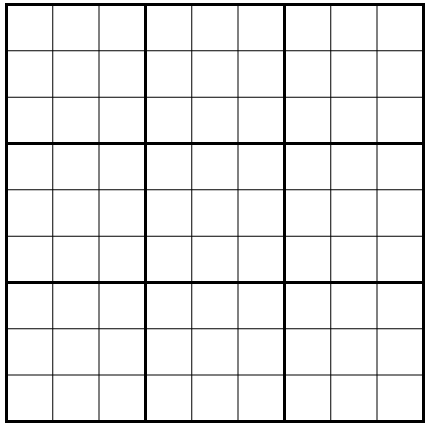
\includegraphics[scale=0.35]{hinh1}
			\caption{\textit{\small Hình $1.$}}
			\vspace*{-5pt}
		\end{figure}
	\end{multicols}
	Sudoku đã xuất hiện ở Pháp vào cuối thế kỷ $19$, nhưng sau đó lại biến mất. Đến năm $1979$, nó xuất hiện trên tạp chí Dell ở Mỹ dưới cái tên Number Place. Sau đó, nó được Nikoli đem về Nhật Bản vào năm $1984$ và đặt cho cái tên  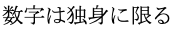
\includegraphics[scale=0.4]{sudoku} (đọc là: Suuji wa dokushin ni kagiru), mà có thể dịch là “các số chỉ được xuất hiện một lần”. Sau này, cái tên này được Maki Kaji viết gọn lại là Sudoku. Từ đó, Sudoku sớm trở thành một trò chơi được ưa chuộng nhất ở Nhật Bản. Mãi cho đến đầu thế kỷ $21$, thế giới mới bắt đầu biết đến Sudoku một cách rộng rãi, khởi đầu từ Anh, sau đó lan sang châu Âu, châu Mỹ.
	\vskip 0.1cm
	Trong bài viết này, trước tiên Bi giới thiệu với các bạn đọc nhỏ tuổi một phiên bản của trò chơi trí tuệ Sudoku; đó là, \textbf{phiên bản hình ảnh}. Phiên bản này rất thích hợp cho các bé từ $5$ đến $7$ tuổi.
	\vskip 0.1cm
	Đối với các bé $5$ hoặc $6$ tuổi, trò chơi sẽ trở nên hấp dẫn hơn, nếu các vị phụ huynh sử dụng thêm các tấm card hình học, hoa quả hoặc bất kì đồ vật gì có sẵn (bút chì, thước kẻ, tẩy, \ldots).
	\vskip 0.15cm
	Giờ, chúng mình cùng Bi trải nghiệm  Sudoku nhé!
	\begin{multicols}{2}
		\textbf{Ví dụ $\pmb 1.$} Vẽ thêm hình vuông, hình tròn hoặc hình tam giác vào các ô vuông còn trống trong bảng ở Hình $2$, sao cho mỗi hình chỉ xuất hiện đúng một lần trong mỗi hàng, cũng như trong mỗi cột.
		\begin{figure}[H]
			\vspace*{5pt}
			\centering
			\captionsetup{labelformat=empty, justification=centering}
			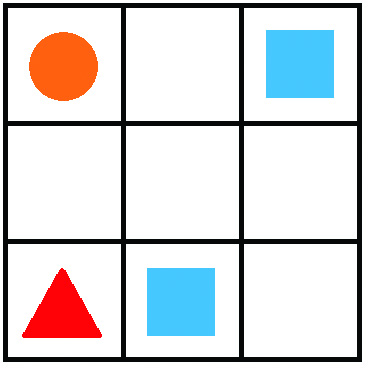
\includegraphics[scale=0.33]{hinh2}
			\caption{\textit{\small Hình $2.$}}
			\vspace*{-10pt}
		\end{figure}
	\end{multicols}
	\textbf{Cùng Bi suy luận:}
	\vskip 0.15cm
	-- Rõ ràng, với mỗi ô còn trống, chúng mình sẽ phải cân nhắc các khả năng điền, rồi lựa chọn hình thích hợp để điền. Vì thế, chúng mình nên bắt đầu từ những ô mà số khả năng điền phải cân nhắc là ít hơn cả, các bé nhỉ? Chúng mình biết rằng, vì trong mỗi hàng, cũng như mỗi cột, phải có đủ cả ba loại hình, nên hình điền ở ô này sẽ “áp đặt” hình nằm ở ô kia. Vì thế, ô trống nằm ở hàng hay cột nào đã có nhiều hình được điền sẽ có số khả năng điền cần cân nhắc ít hơn cả, phải không các bé?
	\vskip 0.15cm
	-- Nhìn bảng ở Hình $2$, chúng mình thấy, có hai hàng và một cột, mà mỗi hàng hay cột đều có sẵn hai hình, nói cách khác, đều chỉ có một ô trống. Với những suy luận ở trên, chắc chắn chúng mình phải bắt đầu từ những ô trống ở hai hàng và cột đó rồi!
	\vskip 0.15cm
	-- Cùng xem nào! Ở hàng trên cùng, đã có hình tròn và hình vuông ở hai ô, vậy thì ở ô trống còn lại chắc chắn phải là hình tam giác rồi! Ở hàng dưới cùng, đã có hình tam giác và hình vuông, nên ở ô trống còn lại chắc chắn phải là hình tròn. Cũng như vậy, ở cột đầu tiên (tính từ trái qua phải), đã có hình tam giác và hình tròn, do đó, ở ô trống còn lại bắt buộc phải là hình vuông.
	\vskip 0.15cm
	-- A ha! Chúng mình đã khám phá ra rồi, nếu trong một hàng hay cột đã có hai ô có hình thì ắt sẽ biết hình phải có trong ô trống còn lại là hình gì.
	\vskip 0.15cm
	-- Với khám phá trên, bằng cách xét các cột thứ hai và thứ ba, chúng mình sẽ dễ dàng điền được hình vào các ô trống còn lại sau bước điền nói trên, phải không nào?
	\vskip 0.15cm
	Các bé xem cách điền hình nêu trên của chúng mình, được thể hiện ở Hình $3$ nhé.
		\begin{figure}[H]
			\centering
			\vspace*{-10pt}
			\captionsetup{labelformat= empty, justification=centering}
			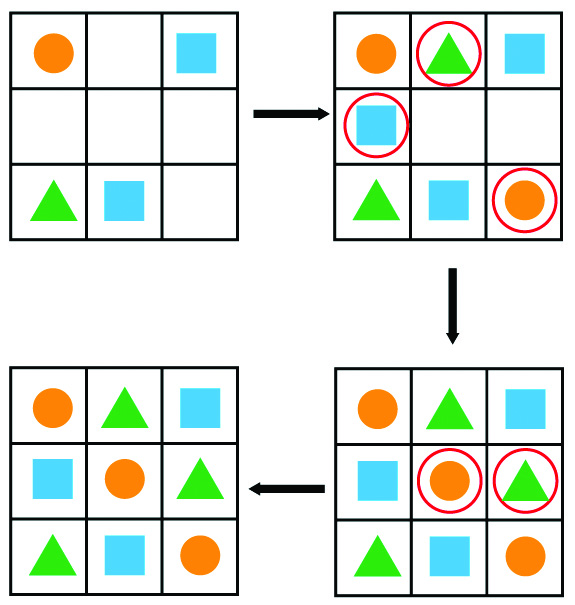
\includegraphics[width=0.48\textwidth]{hinh3}
			\caption{\small\textit{Hình $3.$}}
			\vspace*{-5pt}
		\end{figure}
	Việc giải các sudoku cũng hấp dẫn đấy chứ nhỉ! Giờ hãy cùng Bi thử sức với một sudoku  khác nha!
	\vskip 0.1cm
	\begin{wrapfigure}{l}{0.45\linewidth}
		\vspace*{-10pt}
		\centering
		\captionsetup{labelformat=empty, justification=centering}
		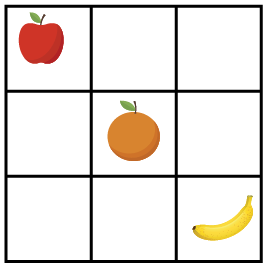
\includegraphics[scale=0.4]{hinh4}
		\caption{\textit{\small Hình $4.$}}
		\vspace*{-15pt}
	\end{wrapfigure}
	\textbf{Ví dụ $\pmb2.$} Vẽ thêm quả cam, quả táo hoặc quả chuối vào các ô vuông còn trống trong bảng ở Hình $4$, sao cho mỗi loại quả chỉ xuất hiện đúng một lần trong mỗi hàng, cũng như trong mỗi cột.
	\vskip 0.1cm
	\textbf{Cùng Bi suy luận:}
	\vskip 0.15cm
	\begin{wrapfigure}{r}{0.45\linewidth}
		\centering
		\vspace*{-5pt}
		\captionsetup{labelformat= empty, justification=centering}
		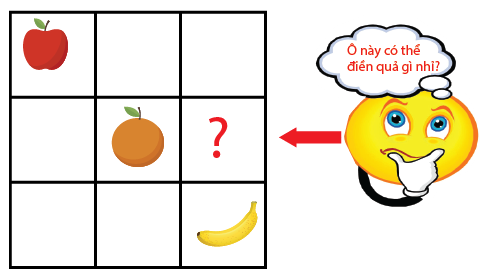
\includegraphics[width=0.45\textwidth]{hinh5}
		%\vspace*{-5pt}
		\caption{\small\textit{Hình $5.$}}
		\vspace*{-5pt}
	\end{wrapfigure}
	-- Quan sát bảng ở Hình $4$, chúng mình không thấy một hàng hay một cột nào, mà ở đó đã có sẵn hai loại quả. Ở hàng nào, cột nào cũng chỉ có đúng một loại quả mà thôi. Thế nghĩa là,  tình huống ở ví dụ này không tương tự như tình huống ở ví dụ $1$ rồi! Phải làm sao bây giờ?
	\vskip 0.1cm	
	-- Suy đi, tính lại, Bi thấy không còn cách nào khác, ngoài cách chọn một ô trống nào đó, rồi cân nhắc các khả năng điền có thể (xem Hình $5$). Các bé có đồng ý với Bi không?
	\vskip 0.1cm
	Hình $6$ thể hiện sự suy xét của Bi khi cân nhắc các khả năng điền đấy. Các bé xem nhé.
	\begin{figure}[H]
		\centering
		\vspace*{-5pt}
		\captionsetup{labelformat= empty, justification=centering}
		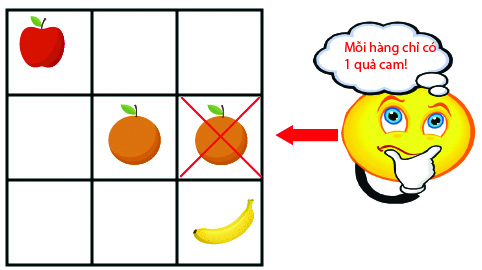
\includegraphics[width=0.3\textwidth]{hinh6a}\hfill
		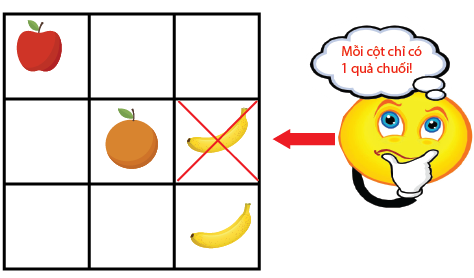
\includegraphics[width=0.3\textwidth]{hinh6b}\hfill
		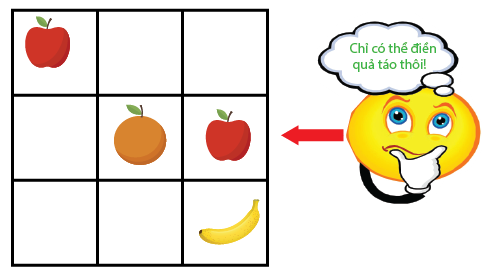
\includegraphics[width=0.3\textwidth]{hinh6c}
		\caption{\small\textit{Hình $6.$}}
		\vspace*{-10pt}
	\end{figure}
	\begin{multicols}{2}
	-- Vui quá, vậy là chúng mình đã cùng Bi điền được quả vào một ô trống rồi (xem Hình $7$).
		\begin{figure}[H]
		\vspace*{-5pt}
		\centering
		\captionsetup{labelformat=empty, justification=centering}
		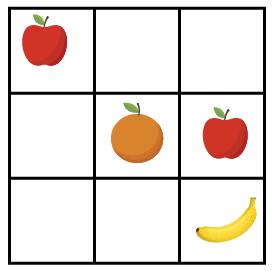
\includegraphics[scale=0.4]{hinh7}
		\caption{\textit{\small Hình $7.$}}
		\vspace*{-5pt}
		\end{figure}
		-- Sudoku trái cây giờ đã trở nên đơn giản hơn, tương tự như ở ví dụ $1$ rồi. Nghĩa là, trong bảng đã có những hàng, những cột mà ở mỗi hàng hay cột đó đều chỉ có một ô trống. Vì thế, bằng các suy luận tương tự như khi giải ví dụ $1$, chúng mình đã có thể tiếp tục điền các loại quả thích hợp vào các ô trống còn lại. Các bé tự làm tiếp nhé.
	\end{multicols}
	\vskip 0.1cm
	Nhìn lại các suy luận ở trên, khi giải ví dụ $2$, Bi nhận thấy rằng, chúng mình điền được quả vào ô trống đầu tiên là do ô đó nằm ở giao của đúng một hàng và đúng một cột, mà ở hàng, cũng như ở cột ấy, lại đã có sẵn một loại quả. A ha, để ý rằng ô nào trong bảng cũng nằm ở giao của đúng một hàng và đúng một cột, chúng mình đã cùng Bi có thêm một khám phá nữa rồi. Đó là, chúng mình sẽ xác định được loại quả nằm ở một ô bất kỳ, nếu biết loại quả nằm trong hàng và trong cột chứa ô đó!
	\vskip 0.1cm
	Hiểu các suy luận của Bi khi giải các ví dụ $1$ và $2$ rồi, bây giờ các bé hãy tập tự mình suy luận để vượt qua các Sudoku dưới đây nhé.
	\vskip 0.1cm
	\textbf{Bài tập $\pmb{1.}$} Vẽ thêm quả đào, quả nho hoặc quả xoài vào các ô vuông còn trống trong bảng ở Hình $8$, sao cho mỗi loại quả chỉ xuất hiện đúng một lần trong mỗi hàng, cũng như trong mỗi cột.
	\vskip 0.3cm
	\begin{figure}[H]
		\vspace*{-5pt}
		\centering
		\captionsetup{labelformat=empty, justification=centering}
		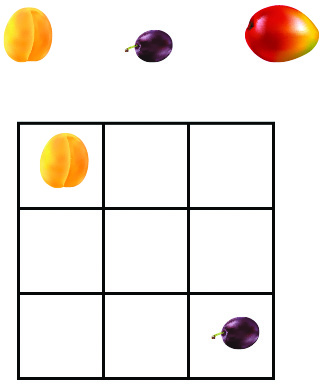
\includegraphics[width=0.30\textwidth]{hinh8}\hspace{40pt}
		%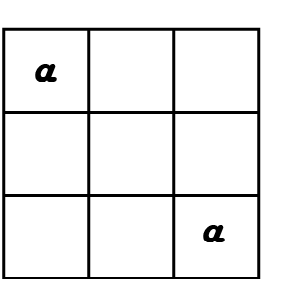
\includegraphics[width=0.25\textwidth]{hinh9}\hfill
		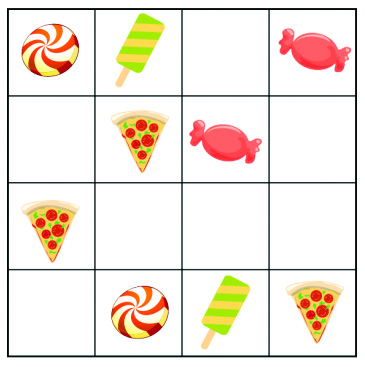
\includegraphics[width=0.30\textwidth]{hinh10}

		\caption{\textit{\small Hình $8.$ \hspace*{100pt} Hình $9.$}} % \hspace*{75pt} Hình 10
		\vspace*{-10pt}
	\end{figure}
	\textbf{Bài tập $\pmb{2.}$} Vẽ thêm que kem, miếng bánh, cái kẹo sữa hoặc cái kẹo ngọt vào các ô vuông còn trống trong bảng ở Hình $9$, sao cho mỗi loại kem, bánh, kẹo chỉ xuất hiện đúng một lần trong mỗi hàng, cũng như trong mỗi cột.
	\vskip 0.1cm
	\textbf{Bài tập $\pmb{3.}$} Vẽ thêm quả cà chua, quả dưa chuột, củ cà rốt hoặc quả cà tím vào các ô vuông còn trống trong bảng ở Hình $10$, sao cho mỗi loại củ, quả chỉ xuất hiện đúng một lần trong mỗi hàng, cũng như trong mỗi cột.
		\begin{figure}[H]
		\vspace*{-5pt}
		\centering
		\captionsetup{labelformat=empty, justification=centering}
		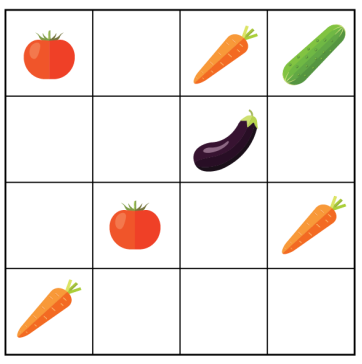
\includegraphics[width=0.3\textwidth]{hinh11}\hspace{40pt}
	%	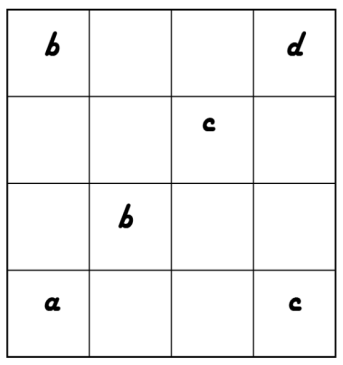
\includegraphics[width=0.3\textwidth]{hinh12}\hfill
		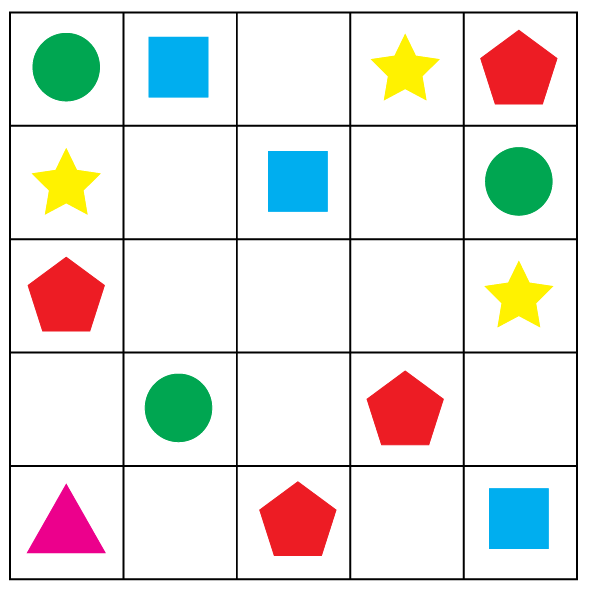
\includegraphics[width=0.3\textwidth]{hinh13}
		
		\caption{\textit{\small Hình $10.$ \hspace*{75pt} Hình $11.$ }}  %\hspace*{75pt} Hình 13
		\vspace*{-10pt}
	\end{figure}
	\textbf{Bài tập $\pmb{4.}$} Vẽ thêm  hình tam giác, hình vuông,  hình ngũ giác, hình ngôi sao hoặc hình tròn vào các ô vuông còn trống trong bảng ở Hình $11$, sao cho mỗi loại hình chỉ xuất hiện đúng một lần trong mỗi hàng, cũng như trong mỗi cột.